\documentclass{article}

\usepackage[top=3cm, bottom=3cm, left=3cm,right=3cm]{geometry}
\usepackage[colorinlistoftodos]{todonotes}
\usepackage{graphicx}
\usepackage{amssymb}
\usepackage{amsmath}
\usepackage{bbm}
\usepackage{todonotes}
\usepackage{pdflscape}
\usepackage{caption}
\usepackage{subcaption}
\usepackage[T1]{fontenc}
\usepackage[utf8]{inputenc}
\usepackage{authblk}
\usepackage{pdfpages}
\usepackage{setspace} 
\usepackage{booktabs}
\usepackage{longtable}
\usepackage{float}
\usepackage{tikz}
\usepackage[colorlinks=true,citecolor=blue, linkcolor=blue]{hyperref}
\usepackage{multirow}
\usepackage{todonotes}
\setlength{\tabcolsep}{5pt}
%%\setlength{\parindent}{0pt}
\usepackage[parfill]{parskip}
\renewcommand{\arraystretch}{1.5}

\renewcommand\Affilfont{\itshape\footnotesize}
\def\ci{\perp\!\!\!\perp}

\renewcommand\Affilfont{\itshape\footnotesize}
\linespread{1.5}

% \usepackage{lineno}
% \linenumbers

% Nature Bibliography style
\usepackage[backend=biber,style=nature]{biblatex}
\addbibresource{library.bib} 

%%%%%%%%%%%%%
%%% Title %%%
%%%%%%%%%%%%%
\title{District-level male medical and traditional circumcision coverage and unmet need in sub-Saharan Africa}

\author{}
\date{}

%%%%%%%%%%%%%%%%%%%%%%%%%%%%%%%%%%%%%%%%%%%%%%%%%%%%%%%%%%%%%%%%%%
%%%%%%%%%%%%%%%%%%%%%%%%%%%%%%%%%%%%%%%%%%%%%%%%%%%%%%%%%%%%%%%%%%
%%%%%%%%%%%%%%%%%%%%%%%%%%%%%%%%%%%%%%%%%%%%%%%%%%%%%%%%%%%%%%%%%%

\begin{document}

%%%%%%%%%%%%%%%%%%%%%%%%%%%%%%%%%%%%%%%%%%%%%%%%%%%%%%%%%%%%%%%%%%
%%%%%%%%%%%%%%%%%%%%%%%%%%%%%%%%%%%%%%%%%%%%%%%%%%%%%%%%%%%%%%%%%%
%%%%%%%%%%%%%%%%%%%%%%%%%%%%%%%%%%%%%%%%%%%%%%%%%%%%%%%%%%%%%%%%%%

\maketitle

\vspace{-1cm}

Patrick O'Toole\textsuperscript{1},
Matthew L. Thomas\textsuperscript{1,2},
Oliver Stevens\textsuperscript{1},
Kevin Lam\textsuperscript{1,3},
Katharine Kripke\textsuperscript{4},
Rachel Esra\textsuperscript{1},
Ian Wanyeki\textsuperscript{5},
Lycias Zembe\textsuperscript{5},
Jeffrey W. Eaton\textsuperscript{1,6} \\
\smallskip
  
\textbf{1} MRC Centre for Global Infectious Disease Analysis, School of Public Health, Imperial Colleg  e London, London, United Kingdom\\
\textbf{2} Department of Earth and Environmental Sciences, University of Manchester, Manchester, United Kingdom\\
\textbf{3} Department of Statistics, University of British Columbia, Vancouver, Canada\\
\textbf{4} Avenir Health, Washington, District of Columbia, United States of America\\
\textbf{5} Joint United Nations Programme on HIV/AIDS (UNAIDS), Geneva, Switzerland\\
\textbf{6} Center for Communicable Disease Dynamics, Department of Epidemiology, Harvard T.H. Chan School of Public Health, Boston, Massachusetts, United States of America\\

\smallskip

* Corresponding Author Email

\clearpage

\begin{abstract}
  \noindent \textbf{Background} \\
  \noindent In 2016, UNAIDS developed a Fast-Track strategy that targeted 90\% coverage
  male circumcision (MC) among men aged 10-29 years by 2021 in priority countries in sub-Saharan 
  Africa (SSA) to reduce HIV incidence. There is substantial variation across subnational 
  regions within countries in both traditional male circumcision (TMC) practices and progress
  towards implementation of voluntary medical male circumcision (VMMC). Tracking progress and
  remaining gaps towards VMMC HIV prevention targets requires detailed district-level circumcision
  coverage data.

  \noindent \textbf{Methods} \\
  \noindent We analysed self-reported data on male circumcision from x nationally representative household
  surveys conducted in x SSA countries between 2006-2020. A spatio-temporal Bayesian
  competing-risks time-to-event model was used to estimate rates of traditional and medical
  circumcision by age, location, and time. Circumcision coverage in 2020 was projected assuming
  continuation of estimated age-specific rates, with probabilistic uncertainty.

  \noindent \textbf{Results} \\
  \noindent Across x countries, from 2010 to 2020 an estimated x million men (x\% CI x-x million)
  were newly circumcised, of whom x million (x - x million) were medically circumcised, and
  x million (x - x million) traditionally circumcised. In 2020, MC coverage among men 10-29
  years ranged from x\% (x\% - x\%) in Zimbabwe (?) to x\% (x\%-x\%) in Togo. MMC coverage
  ranged from x\% (x\%-x\%) in Malawi to x\% (x\%-x\%) in Tanzania, and TMC coverage
  from x\% (x\%-x\%) in Eswatini to x\% (x\%-x\%) in Ethiopia. The largest increase in MMC
  coverage was in Lesotho from x\% to x\%. Within countries, the median difference in MC
  coverage between the districts with lowest and highest coverage was x\%, with the smallest
  variation in Eswatini (x\% to x\%) and largest in Zambia (x\% to x\%). x million men aged
  10-29 need to be circumcised to reach 90\% coverage in all countries.

  \noindent \textbf{Conclusions} \\
  \noindent VMMC programmes have made substantial, but uneven, progress towards male circumcision targets. Granular district and age-stratified data provide information for focusing further programme implementation.

\end{abstract}

\newpage


%%%%%%%%%%%%%%%%%%%%%%%%%%%%%%%%%%%%%%%%%%%%%%%%%%%%%%%%%%%%%%%%%%
%%%%%%%%%%%%%%%%%%%%%%%%%%%%%%%%%%%%%%%%%%%%%%%%%%%%%%%%%%%%%%%%%%
%%%%%%%%%%%%%%%%%%%%%%%%%%%%%%%%%%%%%%%%%%%%%%%%%%%%%%%%%%%%%%%%%%

\section{Introduction}

%%%%%%%%%%%%%%%%%%%%%%%%%%%%%%%%%%%%%%%%%%%%%%%%%%%%%%%%%%%%%%%%%%
%%%%%%%%%%%%%%%%%%%%%%%%%%%%%%%%%%%%%%%%%%%%%%%%%%%%%%%%%%%%%%%%%%
%%%%%%%%%%%%%%%%%%%%%%%%%%%%%%%%%%%%%%%%%%%%%%%%%%%%%%%%%%%%%%%%%%

HIV epidemic continues to to be a problem. Many interventions available etc. VMMC has been proven to be an effective way of doing this. 

The World Health Organization (WHO) and the Joint United Nations Programme on HIV/AIDS (UNAIDS) have identified fifteen countries in sub-Saharan Africa that have a high HIV prevalence and low male circumcision (MC) coverage as priority countries which should scale-up VMMC for HIV prevention: Botswana, Eswatini, Ethiopia, Kenya, Lesotho, Malawi, Mozambique, Namibia, Rwanda, South Africa, South Sudan Tanzania, Uganda, Zambia, and Zimbabwe \todo{Check this and the citations} \cite{UNAIDSJoint, davis2018progress, WHOVoluntary2}. Since 2007, there have been XX\todo{Find this number and cite} million VMMCs conducted in these countries with the support of national governments as well as international organisations such as US President’s Emergency Plan for AIDS Relief (PEPFAR) and the Global Fund to Fight AIDS, Tuberculosis and Malaria. Targets were set by UNAIDS to reach 80\% circumcision coverage among men aged 15--49 years in priority countries by 2015 which have since been updated to reach 90\% circumcision coverage among adolescent boys and young men aged 10--29 years by 2021 \cite{WHOFramework}.

The landscape of male circumcision in sub-Saharan Africa is complex and highly heterogeneous. Despite the upscaling in medical male circumcision (MMC) being a recent phenomenon, it has been long been practised as part of traditional male initiation ceremonies in many African countries. The provision of traditional male circumcision (TMC), such as the typical age at circumcision and what it entails, can vary considerably and is influenced by community, religious, ethnic and cultural led values. There is substantial sub-national heterogeneity in the proportion and average of men receiving TMC between at a district level in South Africa. Even on a national level TMC is universally practiced in {\color{red}\bf XXX} and is barely conducted in {\color{red}\bf XXX}. TMCs conducted during male initiation ceremonies are often performed using non-medical methods non-clinical settings by a traditional practitioner with no formal medical training. The evidence that TMC provides the same HIV prevention benefits as MMC is mixed, due to TMC may not involve a complete circumcision and instead be only partial removal of the foreskin or a simple incision in the prepuce in some populations.  \todo{Cite this paragraph.} 

Why is understanding this important? DMPPT2 and Cork et al. and Thomas et al. have been approaches 

In this paper,...











%%%%%%%%%%%%%%%%%%%%%%%%%%%%%%%%%%%%%%%%%%%%%%%%%%%%%%%%%%%%%%%%%%
%%%%%%%%%%%%%%%%%%%%%%%%%%%%%%%%%%%%%%%%%%%%%%%%%%%%%%%%%%%%%%%%%%
%%%%%%%%%%%%%%%%%%%%%%%%%%%%%%%%%%%%%%%%%%%%%%%%%%%%%%%%%%%%%%%%%%
\newpage
\section{Methods}
\label{sec:orga131cc6}

%%%%%%%%%%%%%%%%%%%%%%%%%%%%%%%%%%%%%%%%%%%%%%%%%%%%%%%%%%%%%%%%%%
%%%%%%%%%%%%%%%%%%%%%%%%%%%%%%%%%%%%%%%%%%%%%%%%%%%%%%%%%%%%%%%%%%
%%%%%%%%%%%%%%%%%%%%%%%%%%%%%%%%%%%%%%%%%%%%%%%%%%%%%%%%%%%%%%%%%%

\subsection{Data}
\label{sec:org020fc8c}

%%%%%%%%%%%%%%%%%%%%%%%%%%%%%%%%%%%%%%%%%%%%%%%%%%%%%%%%%%%%%%%%%%
%%%%%%%%%%%%%%%%%%%%%%%%%%%%%%%%%%%%%%%%%%%%%%%%%%%%%%%%%%%%%%%%%%

Several major survey series included questions on male circumcision status, namely the Demographic and Health Surveys (DHS), AIDS Indicator Surveys (AIS) Population-based HIV Impact Assessment (PHIA) surveys, Multiple Indicator Cluster Surveys (MICS), and, in the case of South Africa, Human Sciences Research Council (HSRC) surveys.

These surveys provided individual-level data on self-reported circumcision status by male respondents, and from this we estimated circumcision rates over time and by type for the years proceeding each survey. The following questions were of interest:
\begin{itemize}
\item The circumcision status of the male individual,
\item The circumcision provider: whether the individual was circumcised by a health worker/professional, traditional practioner, other or unknown,
\item The circumcision location: whether the individual was circumcised at a health facility, in the home of a health worker/professional, at home, at a ritual site, other or unknown
\item The circumcision year, and
\item The date of birth and age at response and circumcision.
\end{itemize}

The age of respondents was calculated from the century-month-code (CMC) of birth and interview dates.
PHIA surveys did not include a question for circumcision location. Circumcisions performed by a medical professional and/or in a medical setting are categorised as MMC. Otherwise, circumcisions are TMC. Where no data is present on location or provider, circumcision type is treated as "Missing". 

Respondents were located to their districts using masked cluster geocoordinates. Where these coordinates were unavailable, as in several MICS surveys, respondents were located to their admin level 1 area hierarchy, most often corresponding to a province. 

Sub-national populations from WorldPop were used to calculate circumcision coverage from circumcision rates. (reference)

\subsection{Model}
\label{sec:org681dda6}

"threemc" (Matt's model for male circumcision) (or "Multi-level model for male circumcision"?) is
a Bayesian, spatio-temporal, competing-risks, time-to-event model (reference). We have extended
this model from its initial application in South Africa to
33
countries within the SSA region. The model produces estimates of circumcision rates, incidence and coverage (i.e. cumulative indidence), with associated uncertainty bounds, stratified by type, year, age and location. Circumcision rates are projected after their most recent household survey
assuming continuation of estimated age-specific rates, with probabilistic uncertainty. Estimates
for single ages were binned into 5-year age groups from 0-4 to 54-59, and other age groups of interest, such as the VMMC target age group of 10-29 year-olds.

A key assumption of the original threemc model was that TMC was constant over time, due to the perceived intransigence in TMC practises and traditional male initiation ceremonies amongst tribal, cultural and religious groups which have developed over time. MMCs amongst paediatric males, defined as those under 10, were also assumed to be constant over time, as VMMC programmes, the  main force behind the adoption of MMC in much of SSA, do not targets males below 10 (reference).

Countries were modelled at the organizational level in which the country team has prioritised their program, called the PSNU area level, or the most granular level available in surveys. Model estimates were weighted by population and post-stratified to produce estimates for their "parent" regions. 

Some additional features were added to threemc during the course of this analysis: 
\begin{itemize}
\item Where no information on circumcision type was available for every survey in a given country, a type-agnostic version of the model was used,
\item Survey estimates for less granular areas were used to inform likelihood estimation for their "child" areas, where previously they were ignored,
\item optional addition of a temporal effect for TMC, due to the suggestion of survey estimates that TMC practices may be changing, even in non-VMMC target countries, over time, and
\item an optional random walk (RW) temporal prior was implemented, where previously only an auto-regressive (AR1) temporal prior was available.
\end{itemize}



\subsection{Model Specification}
\label{sec:orgaf7fa2a}

In our choice of model specification, we were interested in two main assumptions/features of the
model:
\begin{itemize}
\item How we should treat TMC, in terms of whether to continue to assume a constant rate of TMC over time, or to reject that assumption,
\item How to model paediatric MMC, which should be minimal in at least the VMMC target countries.
\end{itemize}

If possible, we hoped to use the same model for every country, or failing that, come up with a
satisfactory choice of model specification which would make sense both qualitatively and
quantitatively. 

Qualitatively, we have made some presumptions about certain countries and their circumcision patterns.
In non-VMMC SSA countries, concentrated in Western and Central Africa (WCA), TMC has historically made up the bulk of MCs.
Therefore, most MMCs in non-VMMC countries are likely to have superseded TMCs performed as part of traditional male initiation ceremonies. This suggests that MMCs in these countries are likely to be on paediatric individuals in traditional settings, so the assumption of constant and
negligible paedaitric MMC could be a poor one. 
Because any increases in MMC will come at the expense of TMC in our "competing-risks" model, it is also plausible that the assumption that TMC rates in these countries have been relatively constant may be unrealistic.
It is therefore likely that the inclusion of a time effect for TMC and not partitioning MMC into adult and time-invariant paediatric rates will be a more realistic reflection of circumcision
patterns in non-VMMC countries.  

Conversely, in VMMC priority countries changes in circumcision patterns have largely been driven by the intervention of VMMC programme implementation. 
As such, it is more realistic to assume that paediatric MMCs are minimal, in line with UNAIDS VMMC policy.
It is more difficult to say whether the rate of TMC will be constant over time in non-VMMC countries.
Historical TMC patterns in these countries, differ significantly, even subnationally.
It may therefore be more realistic to also allow TMC to vary over time in VMMC countries.
In countries where the rate of TMC is stable over time, the model will capture this behaviour, while in countries where TMC varies over time, the inclusion of a time effect for TMC will provide the model with the additional required flexibility to identify this trend.
We would also prefer to not have to treat every VMMC priority country separately with regards to their model specification, so including a time effect for TMC in the models for these countries seems like a logical choice. 

We have also performed a quantitative analysis of the different model specifications available
to us. A more detailed treatment of this can be found in section x of the appendix. 

For each country, we fit a model for each possible model specification for threemc, that is:
\begin{itemize}
\item for each choice of temporal prior, namely AR1, RW1 and RW2,
\item a choice of whether or not to include a paediatric age cutoff for MMC of ten, and
\item a choice of whether to include a temporal effect for TMC.
\end{itemize}
Thus totalling 12 possible models for each country.
These models were fit to all of the survey data available, rather than a subset of the data.
This was because we were most interested here in seeing how the inclusion of a peadiatric age cutoff and/or a temporal TMC effect would effect the fit of the model to the data available, rather than in the relative short-term forecasting ability of the different specifications.
As the choice of temporal prior was more important when forecasting, we were not especially interested in how each of these performed here, but regardless we fit for each temporal prior, for completeness. 

The survey weighted empirical survey circumcision coverage was compared to a sample of 1000 draws from the posterior predictions of circumcision coverage for each country.
Both were aggregated to area level 1 and to five year age groups (from 15-19 through 55-59), to avoid having too many zeros in the survey estimates.

Comparisons were made of mean predictions, using expected log-posterior density (ELPD) and continuous ranked probability scores (CRPS), as well as error statistics such as the mean error (ME), root mean error (RME) and root mean error squared (RMSE).
Also evaluated was the the "calibration" of our model with regards to it's posterior predictive uncertainty.
This involved comparing survey estimates of circumcision coverage with the 50\%, 80\% and 95\% credible intervals (CIs) of our posterior predictive distribution. A "good" calibration was regarded as one in which roughly 50\% of survey observations fell within the 50\% CI range, 85\% within the 85\% CI range, and 95\% within the 95\% range.
Seeing as we were comparing within-sample mean estimates, we were particularly interested in the RMSE of our predictions compared to the survey estimates. 

Just as we distinguished between VMMC and non-VMMC countries when considering the qualitative merits of each model specification, so too did a pattern emerge here when quantitively comparing the model fits for both sets of SSA countries. 

For the non-VMMC countries there was a drastic difference in mean predictive accuracy between the different model specifications.
The best model specification was the model which included a temporal TMC effect, but not a paediatric age cutoff for MMC.
This specification performed the best for x / y countries, averaging a RMSE of x, CRPS of x and ELPD of x, in comparison to the next best specification, ?, which averaged an RMSE of x, CRPS of x and ELPD of x. 
It appeared that the inclusion of a temporal TMC effect was very influential in improving the fit of the model for non-VMMC countries, with specifications including this term averaging a RMSE of x versus x for those which did not include this term.
Models including an MMC paediatric age cutoff of 10 consistently performed worse than other models, averaging an RMSE of x versus x. 
These findings were in line with our previous intuitions on MC patterns in non-VMMC, mainly WCA countries, where TMC was historically high, and increases in MMC are likely within the previously TMC population, and hence MMCs were likely performed on younger individuals than in VMMC countries. 

In contrast, for the VMMC priority countries, the choice of whether to include an MMC paedaitric age cutoff had little effect on model fit.
This may be because under fifteens were not surveyed, and so there were no survey estimates for paediatric populations to compare to our model predictions.
However, the inclusion of this MMC paediatic age cutoff did have a negative effect to the fit for the models to adults for non-VMMC countries, so the fact that it's inclusion here did not hurt model fit suggests it was a more accurate representation of MMC patterns in VMMC priority countries.
As we were aware of VMMC programme policy in not currently circumcising under fifteens, and since it did not seem to negatively effect model fit to adults, we decided to include a paediatric age cutoff of 10 in the model for VMMC coutries. 

Models which including a temporal TMC effect were marginally better, with an average RMSE of x versus x for all other models.
In particular, Kenya, which had high historical TMC in most regions and was the most similar of the VMMC countries to WCA countries in terms of it's circumcision patterns, saw a marked improvement when this effect was included, with an average RMSE of x versus x. For completeness, we decided to include a temporal effect for TMC in the model specification for VMMC priority countries.

It was therefore ultimately decided to include a temporal effect for TMC in the model for both VMMC and non-VMMC countries, while only including a pedaitric age cutoff for VMMC countries.
A table with the full set of fit statistics for each model specification for each country can be found in section x of the appendix.

\subsection{Model Calibration and Choice of Temporal Prior}
\label{sec:orga44afa6}

For some VMMC priority countries, we did not have access to more recent survey data. 
One particular country where this is the case is Tanzania, whose most recent survey was the 2016 PHIA survey.
In these circumstances, there may have been a significant increase in MMC coverage due to VMMC programme implementation which was not captured within our survey period.
VMMC programme data was an available source of more recent circumcision data.
The DMPPT2 model explicitly used this data to estimate MMC. 
The results of DMPPT2, as well as those for countries with more recent surveys who have experienced significant MMC scaleups, suggest that VMMC may have scaled up at a rate not anticipated by threemc where only these older surveys are available.
This was consistent with out-of-sample (OOS) exploration of model fits to countries like Zimbabwe, where removing access to the most recent (2018 DHS) survey similarly underestimates VMMC scale up.
Hence, it was felt that threemc likely underestimates uncertainty with regards to predicting circumcision coverage for progressively later years from our last available surveys, particularly in the case of VMMC priority countries, which have seen rapid increases in historically low circumcision.
A more dramatic "fanning" out of our prediction interval as we forecast further from the last available survey data was therefore deemed desirable, consistent with having greater uncertainty in our future forecasts. 

The two main drivers of uncertainty over time in threemc were:
\begin{itemize}
\item The variance hyperparameters relating to time, including the variance hyperparameters for space-time and age-time interactions, and
\item The choice of temporal prior, for which threemc supports the use of an AR1, RW1 or RW2 prior.
\end{itemize}
The "unpooled" optimised time-related variance hyperparameters for the model fit for each respective country varied significantly, but in general certain patterns and values for these hyperparameters could be associated with a having larger bounds for successive prediction years.

Due to computational constraints, we could not model the entire SSA region together as one singular area hierarchy, which, through partial pooling and the neighbourhood correlation structure inherent in the model, would allow the model to borrow information from countries with a large amount of available data to inform predictions in countries with older and/or fewer surveys.
One alternative to using a partially-pooled model was to use the uncertainty estimates which produce the best predictions for countries with more recent data to inform our uncertainty estimates in countries with less recent survey data available.
To quantitatively explore this hypothesis, we performed an OOS evaluation of the model fit to each country, removing their most recent survey data (or, in the case where there were two surveys in subsequent years, the two most recent surveys) and comparing posterior predictions to the survey-estimated circumcision coverage, as we did with our analysis of different model specifications.
A grid search over sensible variance hyperparameter values from the "naive" threemc fits for each country and temporal prior was employed, to determine the optimal values and temporal prior choice. 
For the AR 1 model, the effect of different time correlation parameters on our uncertainty bounds was determined to be minimal, and in the interests of parsimony, these parameters were ignored in our calibration efforts with this model.

\todo{Finish this write up!}
\todo{Add results! Also add ternary plot}

\section{Results}
\label{sec:orgfc68fc8}
Our data consisted of 109 nationally representative household surveys conducted in 33 SSA countries between 2002 and 2019.
x sub-national areas amongst these coutries were included in these surveys and modelled.
Of these 109 surveys, 104 contained sufficent information on circumcision, as outlined in the Methods section of this paper. 

These remaining surveys consisted of 711,715 individuals respondents from 108 birth cohorts from 1903 to 2016. The sample size per survey ranged from 21,114 in the South Africa 2017 HSRC survey to 1,459 in the Eswatini 2014 MICS survey.

There was significant censoring and missing data even in the remaining surveys. 
Left censoring of circumcision status, analagous to unknown circumcision age, averaged  34.438\% across all surveys, and ranged from 0\% in the Rwanda 2008 DHS survey to 99.408\% in the Niger 2006 DHS survey.
17 surveys had more than 90\% left censoring of circumcision age, with 42 surveys having less than 10\% left censoring.
No information on age at circumcision was present in the 2004 and 2008 Botswana Aids Impact Surveys. This complete left censoring of circumcised individuals meant that threemc could not be fit to Botswana. 
Right censoring of circumcision status, indicating as of yet uncircumcised individuals, averaged 35.299\% across all surveys, ranging from 0.399\% in the The Gambia 2018 MICS survey to 91.432\% in the Eswatini 2006 DHS survey.

On average across all surveys, 1.788\% of respondents did not respond to either the circumcision location or provider question, and so had unknown circumcision type. 
This was lowest in the Burundi 2010 DHS survey, at 0\%, and highest in the South Africa 2002 HSRC survey, at 29.545\%.
5 countries had unknown circumcision type; DR Congo, Guinea, Liberia, Niger and Senegal. 
Amongst these countries, left censoring averaged 98.457\%. 
However, the mean survey circumcision coverage amongst these same countries was 98.457\%, which may explain the relative lack of circumcision information available in their surveys.

In addition to Botswana, Guinea-Bissau, Equitorial Guinea and the Central African Republic were additional SSA countries where we did not have any surveys containing circumcision information, and so we were unable to fit threemc in these countries either. 

More information on individual surveys, including participation rates, can be found in section x of the appendix. 

% Surveys Plot (may be moved to supp. figs)
\begin{figure}
    \centering
    % 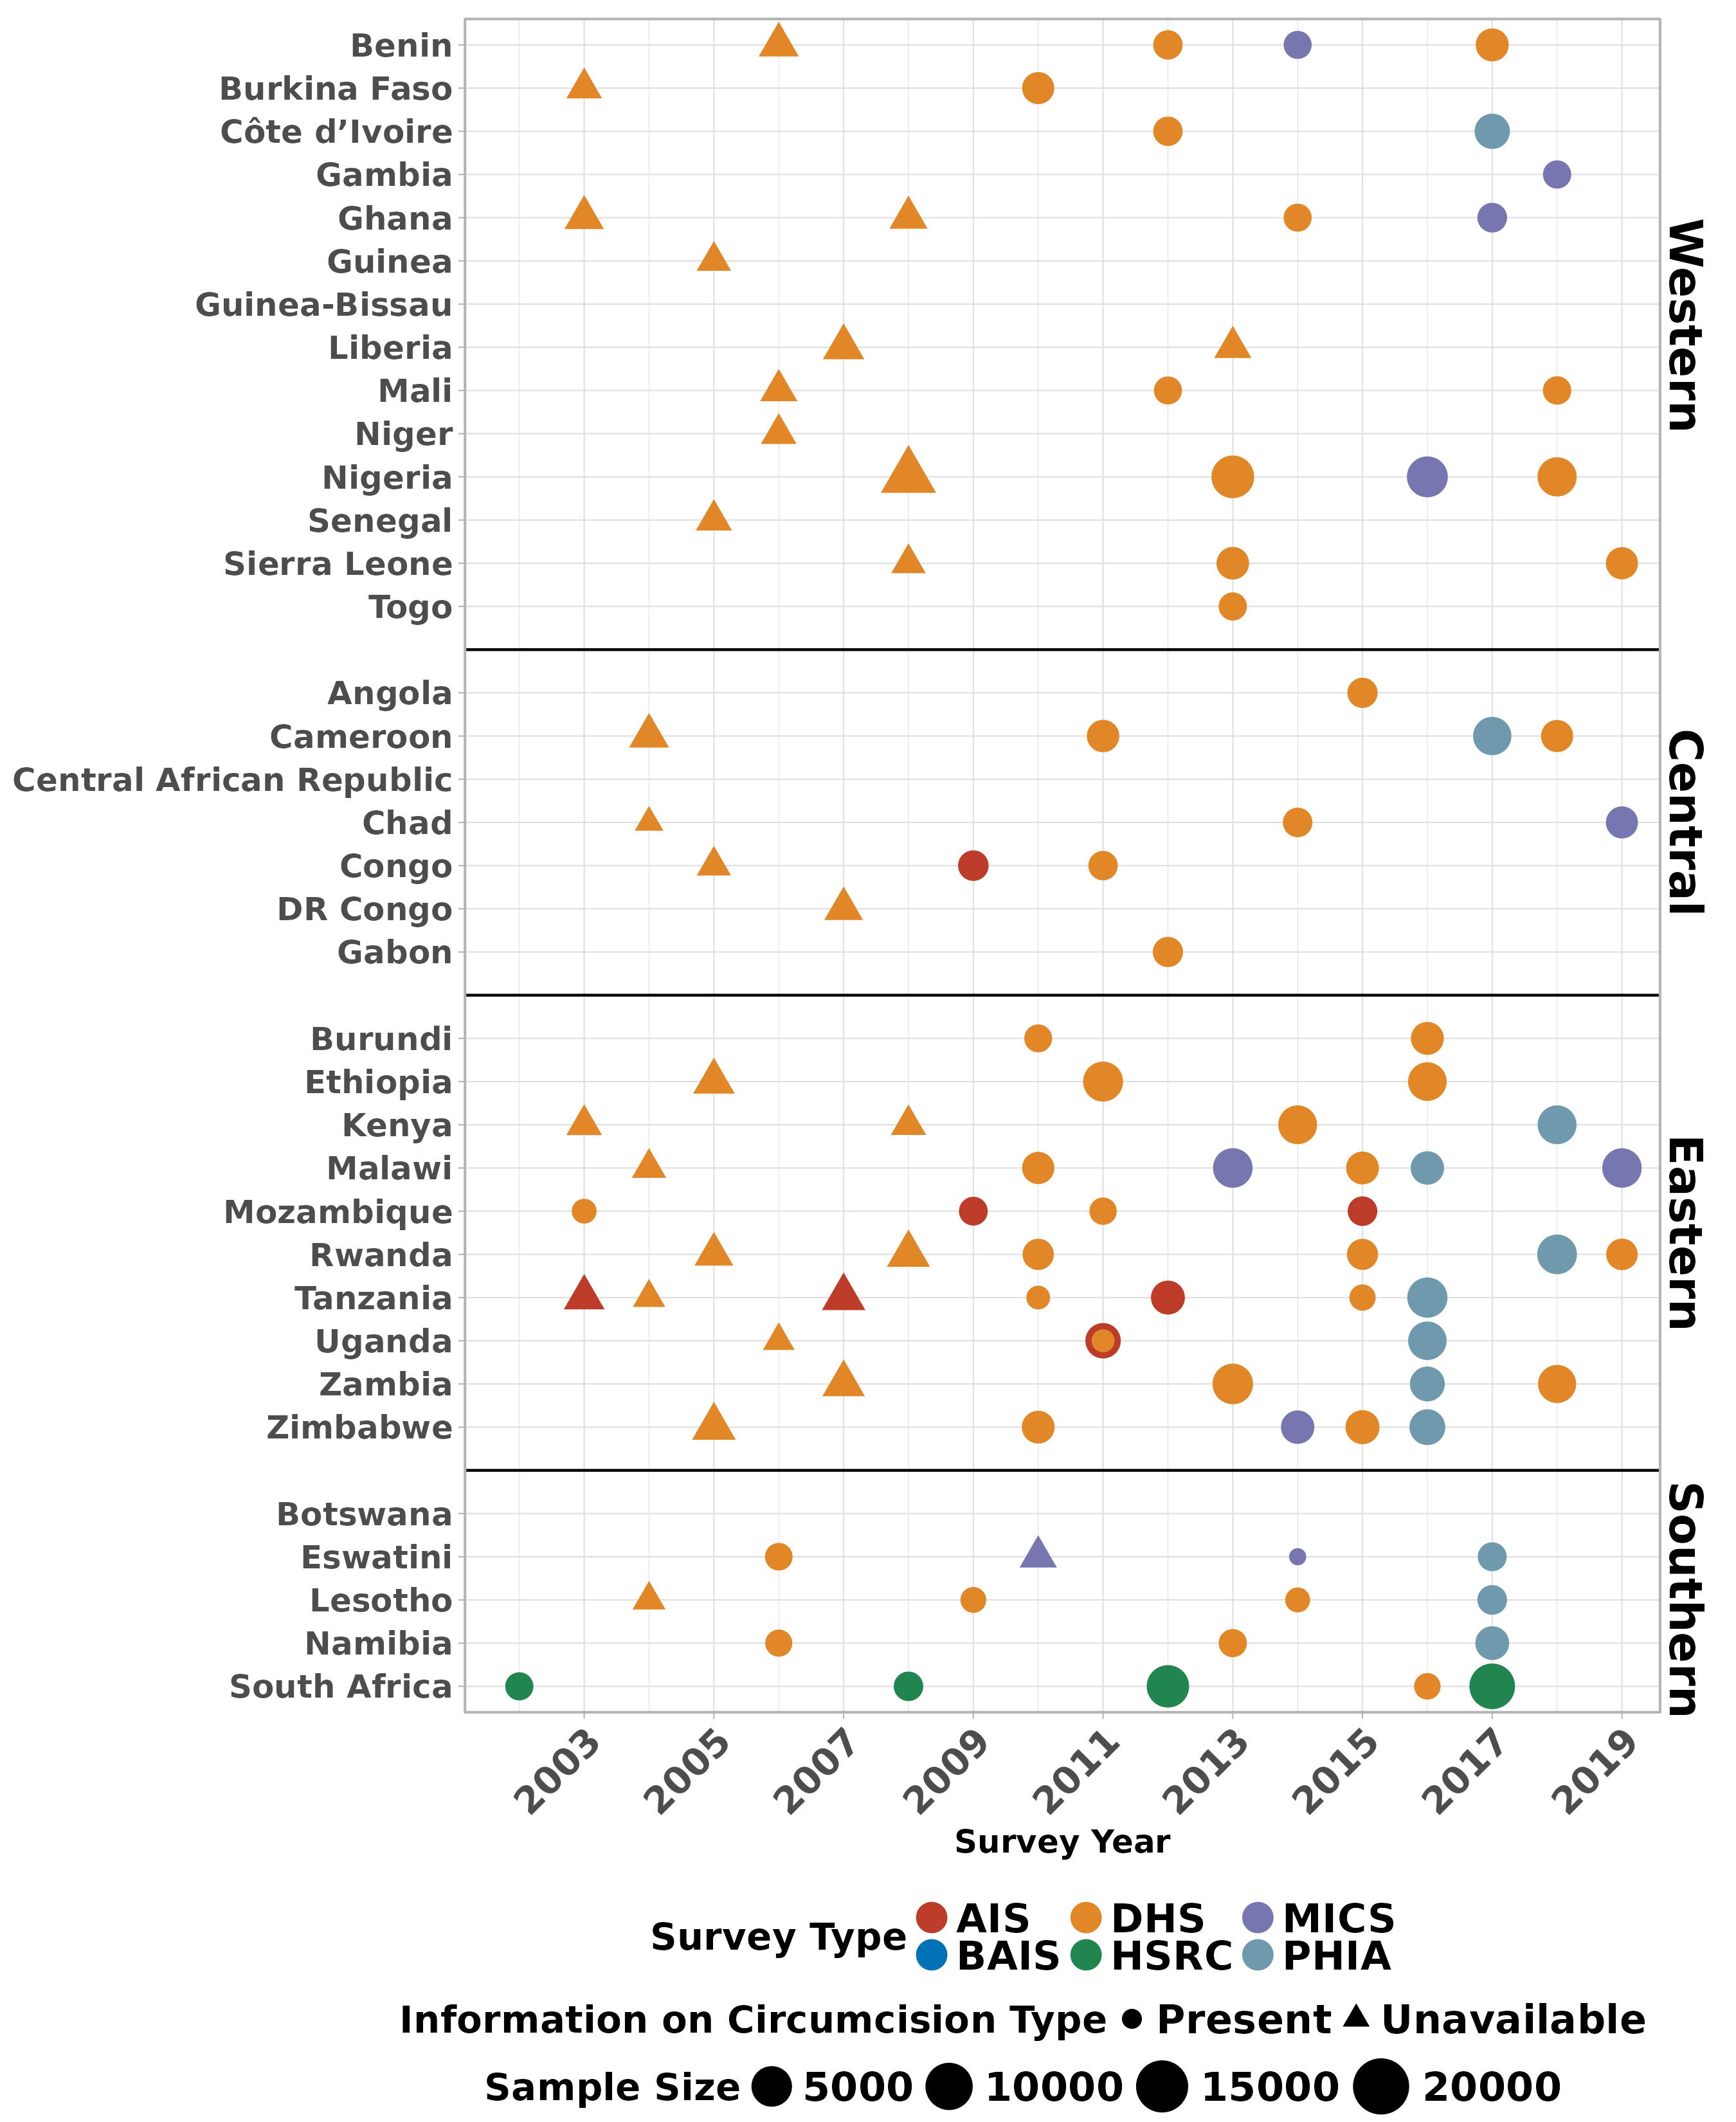
\includegraphics[width=.9\linewidth]{plots/01_survey_table.pdf}
    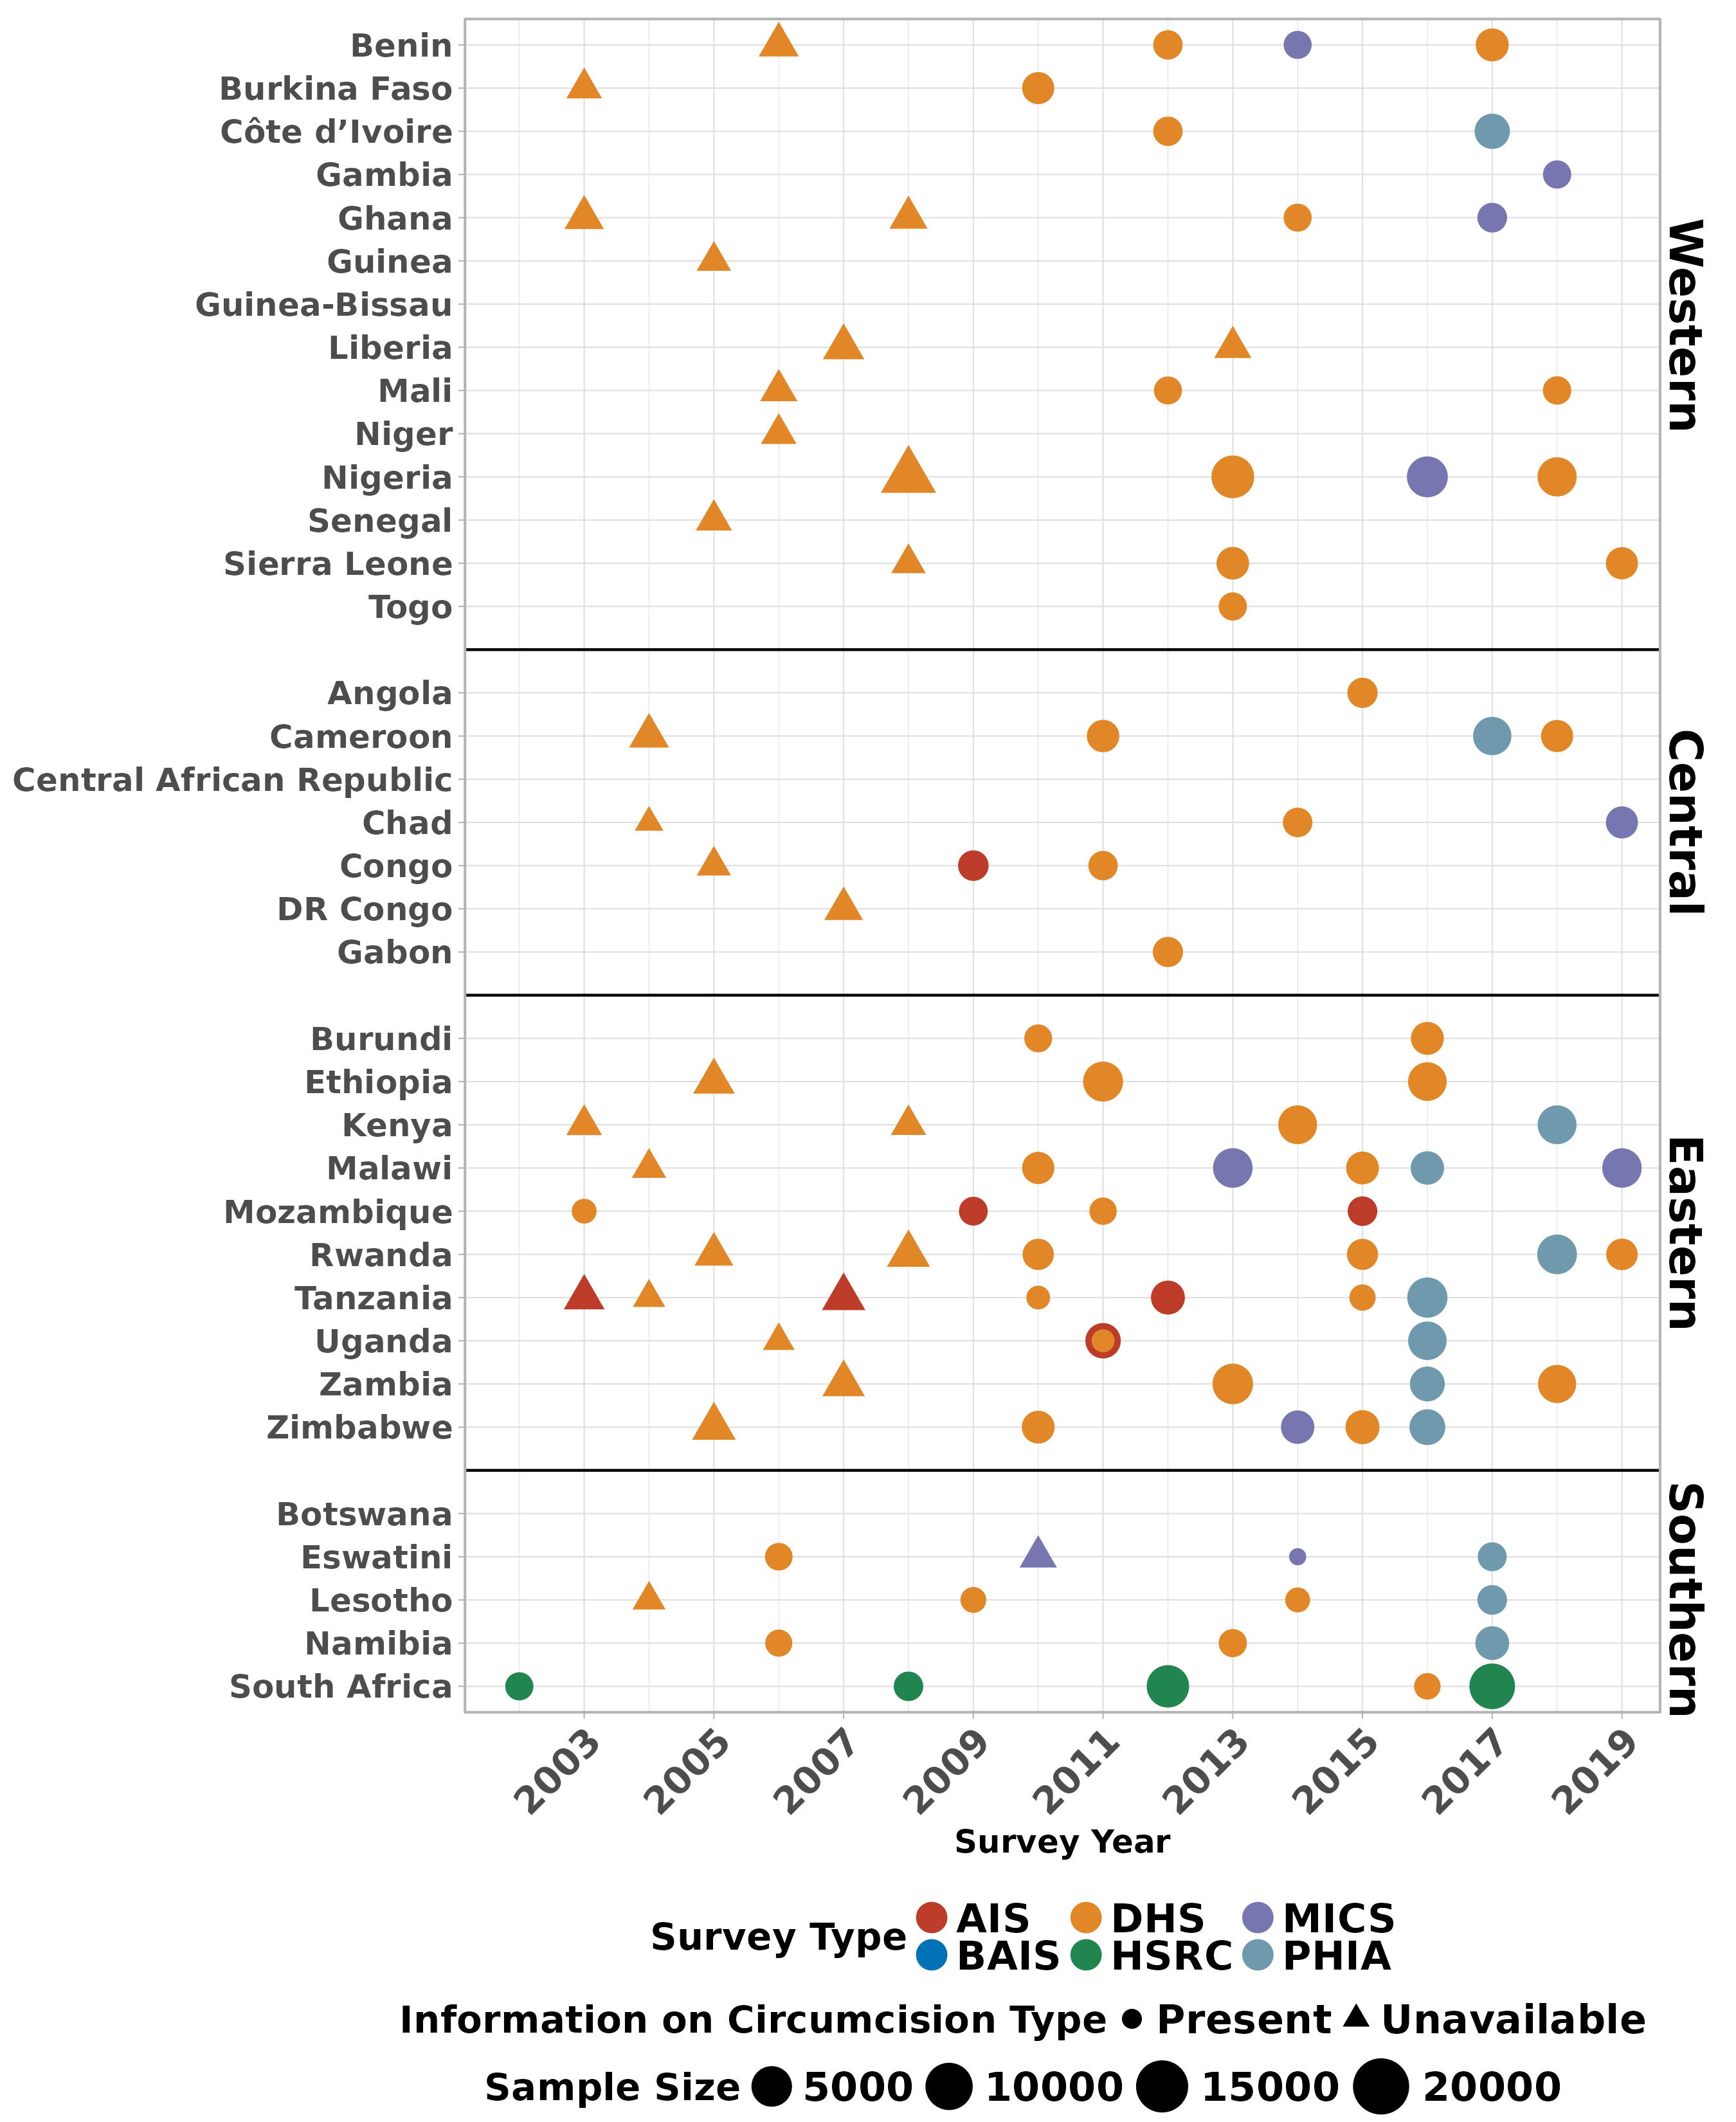
\includegraphics[width=.9\linewidth]
    {plots/01_survey_table.png}
    \caption{\emph{Household surveys detailing circumcision patterns in SSA. The colour and size of points are determined by the provider and sample size of each respective survey. Triangular points have no information on circumcision type.}}
\end{figure}

\subsection{Subnational Variation in Total, Medical \& Traditional Circumcision over time}
\label{sec:org0d1ffe6}

% Map Plot
\begin{figure}
    \centering
    % \includegraphics[width=.9\linewidth]
    \includegraphics[width=1\linewidth]
    % {plots/02_map_plot_facet.png}
    {paper/plots/02_map_plot_facet.png}
    \caption{\emph{Estimated percentage of men aged 10-29 years who were circumcised subnationally in 33 SSA countries in 2006 and 2020, as well as the difference in coverage between the two years. Maps show total male circumcision (MC), medical male circumcision (MMC) and traditional male circumcision (TMC), for which the negative change from 2006 to 2020 is shown, respectively. Missing from map: Guinea-Bissau, Equitorial Guinea, Central African Republic and Botswana}}
\end{figure}
\todo{
  - Use divergent colour palette for "% change", and different one for coverage
- Need to position colour bars under corresponding facets, rather than to the side
- Grey out countries with no type (done)
- reevaluate text size
}

Between 2007, the year VMMC programme implementation began, and 2020, an estimated x million men(95\% CI: x - x million) were newly circumcised. 
Of these, x million (x - x million) were MMCS, along with x million (x - x million) TMCS. 
This translated to an increase in MC for the SSA region of x\% (x\% - x\%) in 2010 to x\% (x\% - x\%) in  2020. 
MC in 2020 ranged from x\% (x\% - x\%) in x to x\% (x\% - x\%) in x, while MMC ranged from x\% (x\% - x\%) in x to x\% (x\% - x\%) in x and TMC ranged from x\% (x\% - x\%) in x to x\% (x\% - x\%) in x. 
The largest percentage increase in MC coverage from 2010 to 2020 was x\% (x\% - x\%) in x, from x\% (x\% - x\%) to x (x\% - x\%), while for MMC it was x\% (x\% - x\%) in x. 
The number of annual MCs performed increased from x (x to x) in 2006 to x (x to x) in 2020, a growth of x (x to x) annually. 
Amongst these, x (x to x) were MMCs in 2006, while in 2020 x (x to x) MMCs were performed, representing an increase in x (x to x) in MMCs performed annually. 
TMC did not increase anywhere,  and actually decreased in several countries from 2010 to 2020. 
This is the focus of a later section of our results. 

For VMMC countries, MC increased from x\% (x\% - x\%) to x\% (x\% - x\%), largely driven by an increase in MMC from x\% (x\% to x\%)  to x\% (x\% - x\%). 
In constrast, for the non-VMMC countries, MC increased from x\% (x\% - x\%) to x\% (x\% - x\%), with MMC going from x\% (x\% to x\%)  to x\% (x\% - x\%). 
TMC in 2020 for VMMC countries averaged x\% (x\% - x\%), compared to x\% (x\% - x\%) in non-VMMC countries. 

Increases in MC coverage from 2010 to 2020 were very heterogeneous, with VMMC programmes generally targeting subnational regions where HIV burden is high and where VMMC as a HIV prevention method is better acknowledged (ref. 42 in Matt's paper)
In ESA countries, MC in 2010 averaged x\% (x\% - x\%). 
This increased to x\% (x\% - x\%) in 2020. MMC increased from x\% (x\% - x\%) in 2010 to x\% (x\% - x\%) in 2020. 
In constant, in WCA MC in 2010 averaged x\% (x\% - x\%), while in 2020 it averaged x\% (x\% - x\%).
MMC in WCA increased from x\% (x\% - x\%)
2020 TMC in ESA countries averaged x\% (x\% - x\%), compared to x\% (x\% - x\%) in WCA countries. 

% Subnational coverage plot
\begin{figure}
    \centering
    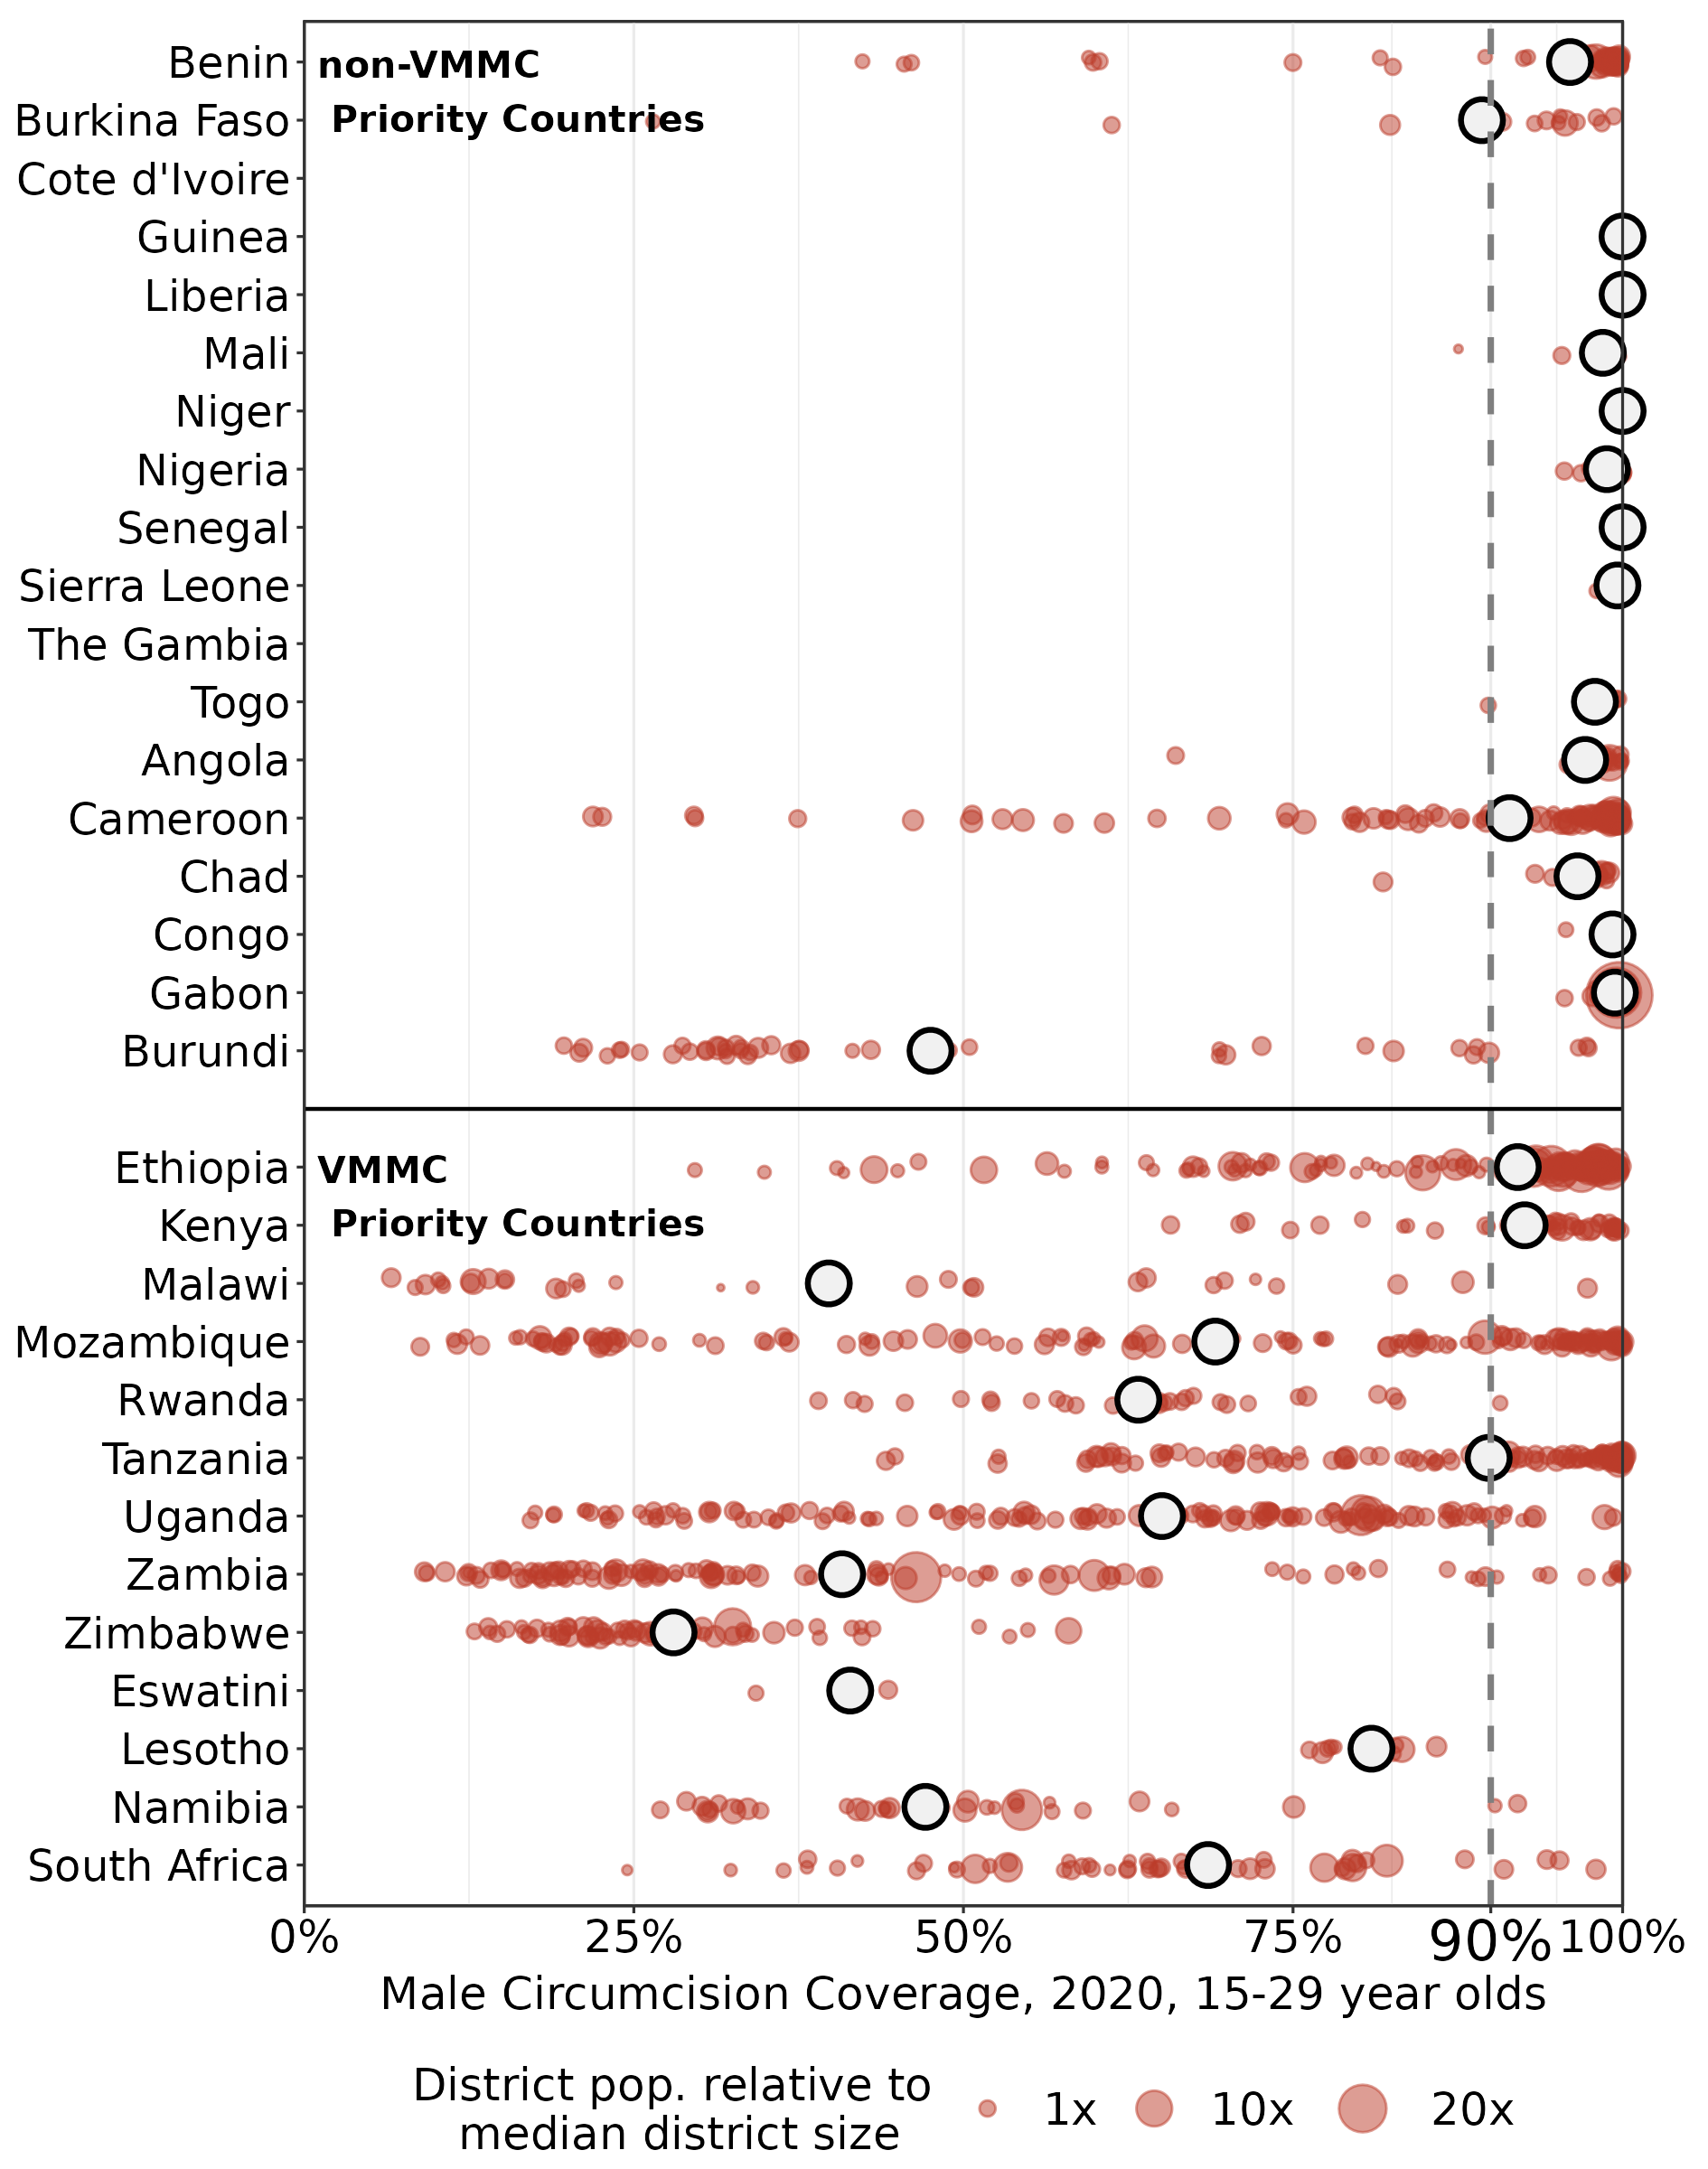
\includegraphics[width=.9\linewidth]
    {plots/03_subnat_plot.png}
    \caption{\emph{District-level median percentage of men aged 10-29 years who were circumcised in 2020 in 33 SSA countries.
    Each point is a district, sized by district population relative to average district size and coloured by the African region their country falls under (Eastern and Southern Africa (ESA) and Western and Central Africa (WCA), respectively).
    Each white dot represents the national median. A vertical dotted line signifies the UNAIDS target of 90\% national MC.}}
\end{figure}


Within countries, the median difference in MC coverage between the districts with lowest and highest coverage in 2020 was x\% (x\% - x\%).
For ESA countries, this was x\% (x\% - x\%), in contrast to WCA countries, where it was x\% (x\% - x\%).
The largest variation overall (and ESA) was in x, from x\% in x to x\% in x, while the largest variation for WCA countries was x, from x\% in x to x\% in x. 
In total, the mean percentage of districts in each country with greater than 90\% MC coverage amongst those aged 10-29 was x\%. In ESA, this was x\%, while in WCA, this was x\%. 

\subsection{Subnational Variation in Total, Medical \& Traditional Circumcision Across Different Ages}
\label{sec:org92e0f37}

% Geofaceted plot of 2020 coverage by age
\begin{figure}
    \centering
    
\includegraphics[width=.9\linewidth]
    {plots/04_geo_age.png}
    \caption{\emph{Projected percentage of men from 0 to 60 years old who were medically circumcised and traditionally circumcised by 2020. The horizontal grey dashed line indicates the 90\% circumcision coverage by 2021 target established by the UNAIDS Fast Track strategy. Purple areas represent countries where circumcision type could not be ascertained from surveys.}}
\end{figure}


Age at circumcision differed greatly by circumcision type and location. 
The age group which experienced the greatest increase in MC coverage from 2006, the year before VMMC programme implementation began (reference), to 2020 was x, reflecting VMMC focus on these ages. 
The age group with the highest MC coverage in 2020 was x, in contrast to 2006, where this age group was x. 
The age group with the highest MMC coverage in 2020 was x, while for TMC coverage this age group was x. 
The average age of MC in 2020 in SSA was x, compared to x in 2006. 
For MMC, the average age at circumcision in 2020 was x, compared to x in 2006, while for TMC the average age was x in 2020, compared to x in 2006. 
The average age of MC in 2020 for ESA was x, while in WCA it was x. 

\subsection{Decrease in TMC in SSA region Over Time}
\label{sec:org5fb5e18}

% Dumbbell of type-specific cov change 00'-20'
% todo: Rewrite caption
\begin{figure}
    \centering
    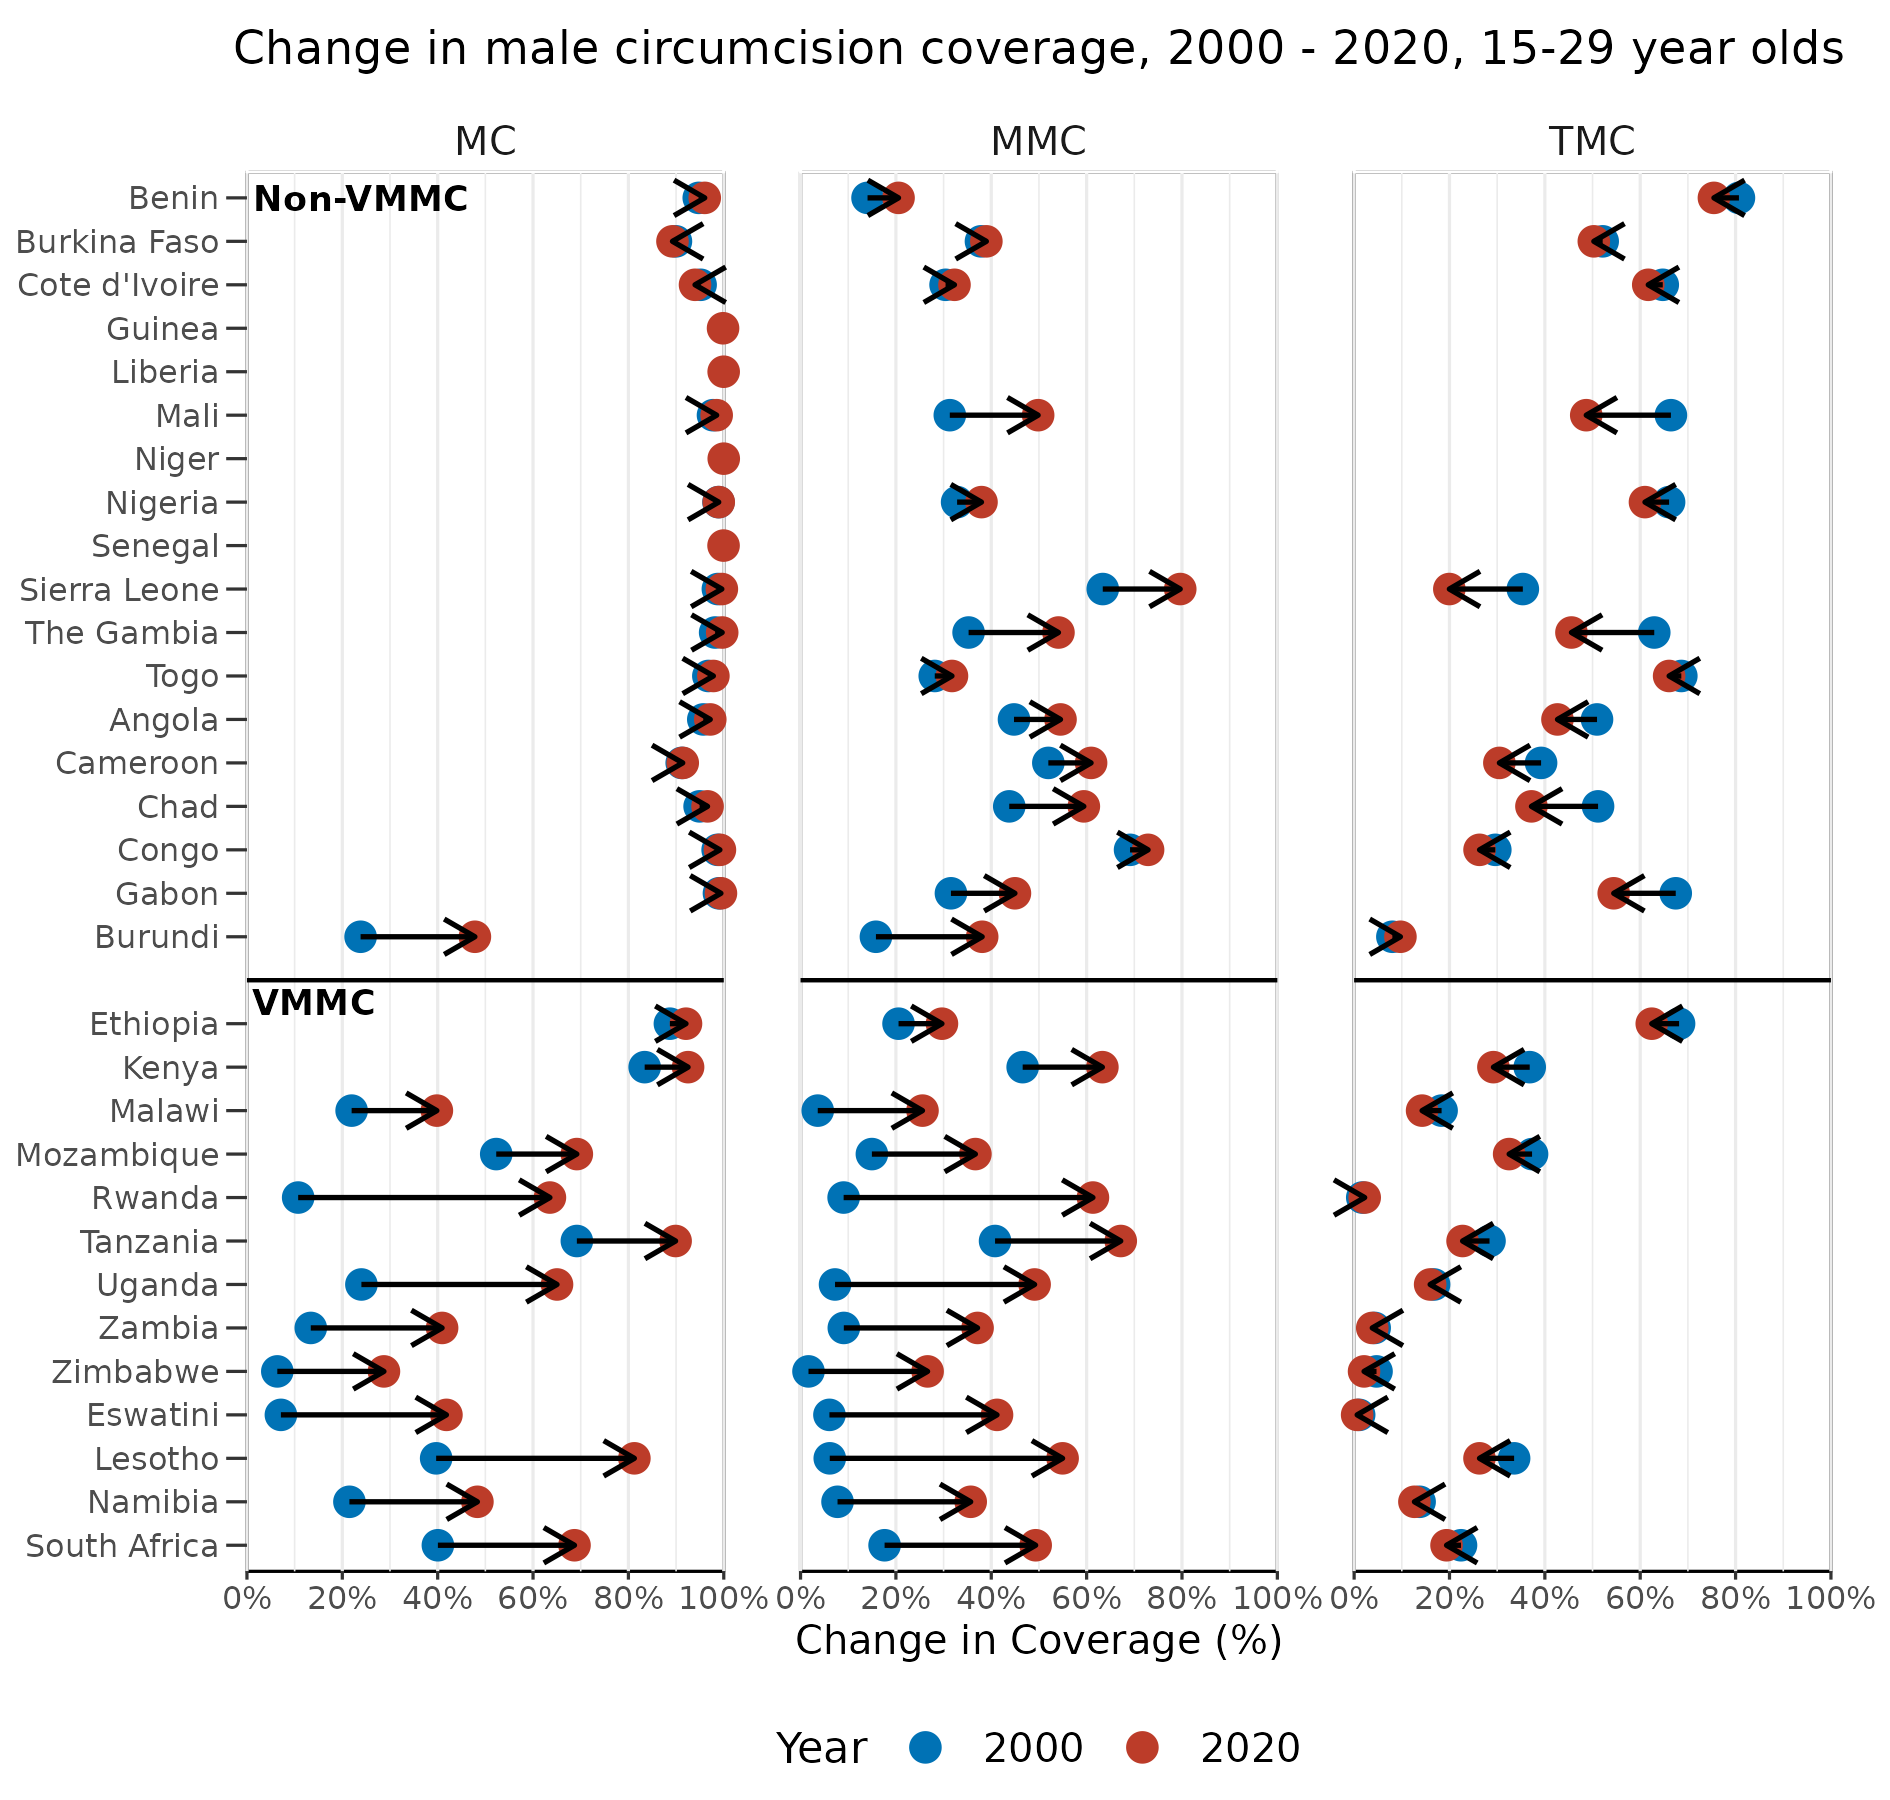
\includegraphics[width=.9\linewidth]
    {plots/05_change_00_20.png}
    \caption{\emph{Absolute difference, with associated errors, in percentage coverage from 2000 to 2020, coloured by sub-Saharan African region. Plots are split by circumcision type. Countries are ordered from north to south, east to west, and the 13 countries below the black horizontal lines are VMMC priority countries.  }}
\end{figure}

The average TMC coverage in SSA in 2006 was x\% (x\% to x\%). 
This fell to x\% (x\% to x\%) in 2020, representing a decrease of x\% (x\% to x\%). 
In ESA, TMC coverage was x\% (x\% to x\%) in 2006, compared to x\% (x\% to x\%) in 2020, a x\% (x\% to x\%) decrease. In constrast, TMC coverage in WCA was x\% (x\% to x\%) versus x\% (x\% to x\%) in 2020, a x\% (x\% to x\%) fall. 
In 2006, x (x to x) TMCs were performed, while in 2020 this was reduced to x (x to x), representing a x (x to x) decrease in annual TMCs.
In ESA, the annual number of TMCs performed dropped from x (x to x) in 2006 to x (x to x) in 2020, a x (x to x) drop. 
In WSA, this number fell from x (x to x) in 2006 to x (x to x) in 2020, a fall of x (x to x).
For the 10-29 age group, TMC coverage was reduced from x\% (x\% to x\%) in 2006 to x\% (x\% to x\%) in 2020, a drop of x\% (x\% to x\%).
In VMMC countries, this was reduced from x\% (x\% to x\%) to x\% (x\% to x\%) from 2006 to 2020, while even in non-VMMC countries this decreased from x\% (x\% to x\%) to x\% (x\% to x\%). 
The largest decrease in TMC coverage from 2006 to 2020 was in x, from x\% (x\% to x\%) to x\% (x\% to x\%). 
[If the above is a VMMC country] The largest decrease in TMC coverage amongst non-VMMC countries was from x\% (x\% to x\%) to x\% (x\% to x\%) in x. 

\subsection{UNAIDS Goals Progress amongst 10-29 Year Olds in VMMC Target Countries}
\label{sec:orgf9204d9}

Amongst the 13 VMMC priority countries modelled, just x countries were projected to have achieved the VMMC target of 90\% MC coverage amongst 10-29 year olds, x and x. 
MC coverage across these countries increased from x\% (x\% to x\%) in 2006 to x\% (x\% to x\%) in 2020. 
X (x to x) circumcisions were performed between 2007 and 2020 in these countries. 
Of these, x (x to x) were MMCs. 
No countries were expected to have reached this goal in all districts. 
The number of annual MCs increased from x (x to x) in 2006 to x (x to x) in 2020. 
x (x to x) additional circumcisions are required to achieve 90\% MC coverage in all VMMC countries, x (x to x) times the projected number of MCs for 2020. 
The largest increase in MC coverage amongst VMMC priority countries was in x, from x\% (x\% to x\%) in 2006 to x\% (x\% to x\%) in 2020, a x\% (x\% to x\%) increase. 
In contrast, the lowest increase in MC coverage in these countries was in x, from x\% (x\% to x\%) in 2006 to x\% (x\% to x\%) in 2020, a x\% (x\% to x\%) increase. 

However, these figures belie significant subnational heterogeneity in MC coverage amongst VMMC prioirty countries. 
x/x districts in these countries were expected to have reached 90\% MC coverage amongst 10-29 year olds in 2020, up from x/x in 2006, before VMMC programmes began. 
Even in x, where MC was projected to be lowest in 2020, x/x districts were forecasted to have reached 90\% MC coverage for men aged 10-29 years old. 
MC coverage there increased from x\% (x\% to x\%) in 2006 to x\% (x\% to x\%) in 2020, a x\% (x\% to x\%) increase. 

TODO: Add some kind of table here!

\subsection{Comparison to results of DMPPT2 model}
\label{sec:orge0178ca}

TODO: Write this section!

\section{Discussion}
\label{sec:orgca35e01}

Sub-national MC has increased significantly from 2006 to 2020. 
However, there is sharp national and sub-national differences in MC coverage and type. 
Despite this, some obvious regional patterns can be observed to have emerged over this time period. 
Broadly speaking, WCA has much higher MC coverage, in line with greater cultural practice of TMC associated with these countries. 
MC coverage is generally more homogeneous in WCA countries. 
Even in WCA, where VMMC programmes have not been implemented, there has been significant growth in the number of MMCs peformed. 
In contrast, in ESA MC and particularly TMC coverage is generally lower, although this varies substantially, both nationally and sub-nationally. 
This variability may in part be attributed to efforts to focus VMMC programmes on areas of high disease burden and a lack of historical TMC practice. 
However, there have been significant increases in MC coverage in ESA as a result of VMMC programme implementation in many of these countries.

Since 2006, MMCs have increased significantly for younger ages, particularly amongst the 10-29 age group which has been focused on by VMMC implementation. 
A circumcised individual is much more likely to have undergone MMC for progressively younger ages, while the converse is true for TMC.
Over time, this pattern has become more pronounced, particularly amongst VMMC countries. 

TODO: Flesh this out! Mention how this differs for VMMC and non-VMMC countries, and maybe there is some pattern for TMC-MMCs?

TMC has decreased, both in VMMC target countries and elsewhere. 
In priority countries, this is presumably largely due to the implementation of VMMC programs in districts which traditionally practised TMC. 
It is interesting that TMC has also also, non-uniformely, declined in many countries and regions elsewhere in SSA. 
This could possibly be in response to general economic upliftment and development in these countries, and an increased willingness to accept VMMC as an effective, cheap HIV prevention strategy. 

Significant, but uneven progress has been made towards achieving the UNAIDS target of 90\% 
MC coverage amongst 10-29 year olds in 14 VMMC priority countries by 2021.  
However, this has resulted in just x country, x, expected to have realised this goal.
Granular district and age-stratified estimates for MC, as provided by threemc, provide a key source of information for focusing further programme implementation in these VMMC priority countries, in addition to subnational HIV burden estimates which identify the areas most in need of HIV prevention interventions such as VMMC. 

In the majority of VMMC countries, the results of threemc and DMPPT2 largely agree. 
However, for several countries, namely Tanzania, Zimbabwe and parts of Kenya, we can see that DMPPT2 estimates far exceed empirical survey and threemc estimates, and indeed the population of many districts, suggesting that they may be adversely affected by 
\begin{enumerate}
\item people travelling from their home districts to others to avail of VMMC programmes, and
\item ii) possible misreporting occurring in programmatic data due to incentives to report higher numbers of circumcisions for VMMC clinics.
\end{enumerate}
Where it is desired to incorporate VMMC programme data in estimates of MC coverage, threemc may provide a useful "baseline" circumcision estimate for DMPPT2 up until the last household survey was performed, with programme data taking over as the main data source thereafter.  
threemc may also complement DMPPT2 in it's inclusion of estimates for TMC, since DMPPT2 and the programme data only concern MMC. 

There were several limitations inherint in the threemc model, and in this analysis. 
TODO: Write these out!
There is much scope for further developments from this analysis. 
One obvious, though difficult possibility is the incorporation of programme data within threemc. 
Efforts to do so in South Africa were successful in the original threemc paper, but further implementation of the model including programme data in Malawi has struggled to ? survey and programme data. 
In the face of these difficulties, a viable compromise may be to use threemc to provide baseline MC and estimates for TMC to the DMPPT2 tool, as described above. 
The results of this analysis can also provide circumcision coverage covariates to eligible models which seek to estimate and predict HIV incidence and prevalence, such as Naomi. 
Finally, we hope that threemc can continue to incorporate new household surveys as they become available, which will be useful for both providing new circumcision estimates, and validating current predictions. 
In particular, a new DHS survey is expected for Botswana in ?, a welcome development which will allow the model to be extended to this VMMC priority country. 

TODO: Good conclusion of one line?

\section{Availability of data and materials}
\label{sec:orgd999c87}
\subsection{Data Availability}
\label{sec:org953a659}
\subsection{Code Availability}
\label{sec:org2a96da6}
threemc is implemented in an R package, which can be found on Github at \url{https://github.com/mrc-ide/threemc}. The code used to generate the results of this paper is located at \url{https://github.com/mrc-ide/threemc-orderly}, and makes heavy use of the orderly R package [include reference!].
\end{document}